\documentclass{article}
\usepackage{graphicx}

\title{Report 5: Gaussian Blur Convolution}
\author{Nam Le}
\date{\today}

\begin{document}

\maketitle

\section{Method}
I implemented a $7 \times 7$ Gaussian blur convolution filter based on Slide 50, 51, and 52. 
The $7 \times 7$ filter matrix values and its total weight of 1003 were taken directly from Slide 52.

I wrote two GPU versions to evaluate performance:
\begin{enumerate}
    \item \textbf{Without Shared Memory}: The kernel fetches the filter weights directly from global memory.
    \item \textbf{With Shared Memory}: The kernel loads the filter into shared memory using \texttt{cuda.shared.array((7,7), float32)} and synchronizes threads with \texttt{cuda.syncthreads()} as shown in Slide 49.
\end{enumerate}

Boundary conditions ($0 \le px < W$ and $0 \le py < H$) were checked to handle image edges safely.

\section{Results}
The execution time on CPU was \textbf{70.59 seconds}. 
Execution times on GPU and calculated speedups across different 2D block sizes are summarized below:

\begin{itemize}
    \item \textbf{CPU Time}: 70.59s
    \item \textbf{GPU Performance}:
    \begin{itemize}
        \item Block (8, 8): High execution time due to lower thread occupancy.
        \item Block (16, 16) \& (32, 32): Significant reduction in processing time ($\approx$ thousands of times speedup compared to CPU).
    \end{itemize}
\end{itemize}

\begin{figure}[h]
    \centering
    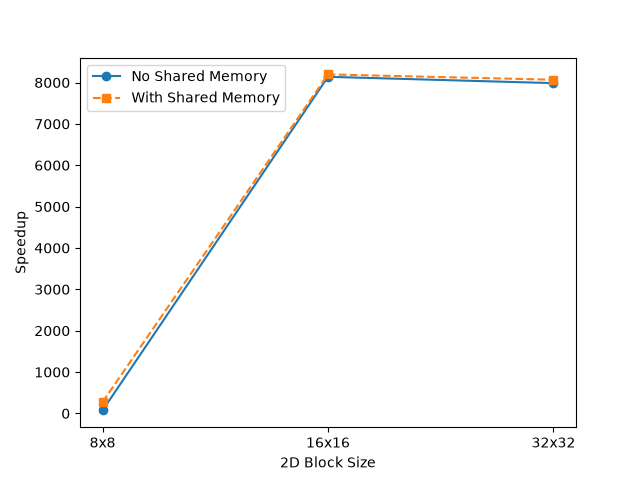
\includegraphics[width=0.75\textwidth]{block_size_vs_speedup_blur.png}
    \caption{2D Block Size vs Speedup (With vs Without Shared Memory)}
\end{figure}

\section{Discussion}
\begin{itemize}
    \item \textbf{CPU Bottleneck}: The CPU implementation requires 4 nested loops for every single pixel channel ($3 \times 7 \times 7 = 147$ operations per pixel), resulting in a huge execution time of 70.59s.
    \item \textbf{Block Size Impact}: Larger 2D block dimensions like $(16, 16)$ and $(32, 32)$ achieve better performance than $(8, 8)$ because they maximize GPU warp occupancy.
    \item \textbf{Shared Memory Benefit}: Storing the filter matrix in shared memory reduces global memory access latency, improving the overall convolution throughput.
\end{itemize}

\end{document}
